\documentclass[a4paper,twocolumn]{article}
% \pagestyle{empty}

\title{Progetto finale Reti Logiche}
\author{Luca De Martini}
\date{}

% \usepackage[margin=2cm]{geometry}
% \usepackage[hidelinks]{hyperref}
\usepackage[table]{xcolor}
\usepackage{array,multicol,graphicx}
\usepackage[activate=true,final,tracking=true,kerning=true,spacing=true]{microtype}
\microtypecontext{spacing=nonfrench}

\begin{document}

\setlength\parindent{0pt}
% \hyphenpenalty=1500
\emergencystretch 3em

\maketitle
% \begin{multicols*}{2}
    
\section{Introduzione}

\section{Architettura}
Al livello più alto il componente presenta un modulo \texttt{project\_reti\_logiche} che contiene tutti i moduli interni, un'automa a stati finiti e un registro di cache dell'indirizzo in output.

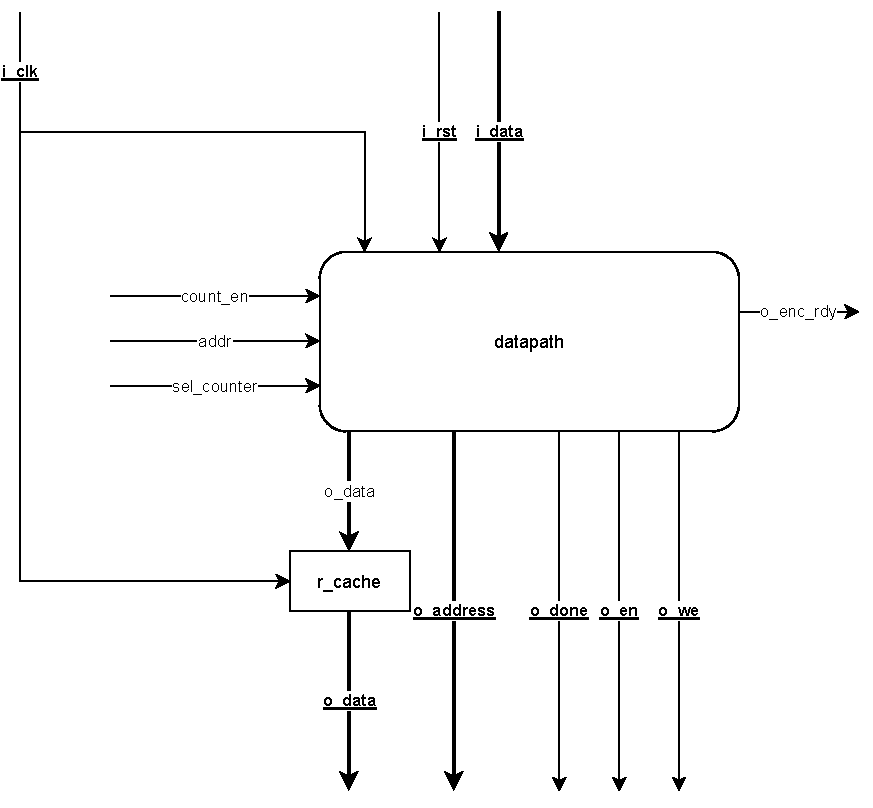
\includegraphics[width=\linewidth]{schema-main.pdf}

L'automa a stati finiti è implementato con una collezione di process:

Due process descrivono il comportamento del registro di cache e quello del registro di stato, entrambi sono realizzati con flip-flop sincroni attivati sul fronte di discesa, la scelta di usare il falling edge è stata fatta per ridurre il numero di cicli di clock necessari per la codifica.

Un altro process aggiorna il valore del segnale \texttt{next\_state} in base allo stato attuale, al segnale in input di \texttt{i\_start} e al segnale \texttt{enc\_rdy}, output del modulo interno \texttt{datapath} che verrà descritto nel dettaglio successivamente.

Infine un ultimo process aggiorna i valori dei segnali in input ai moduli interni e in output dal componente necessari al funzionamento basandosi sullo stato attuale.

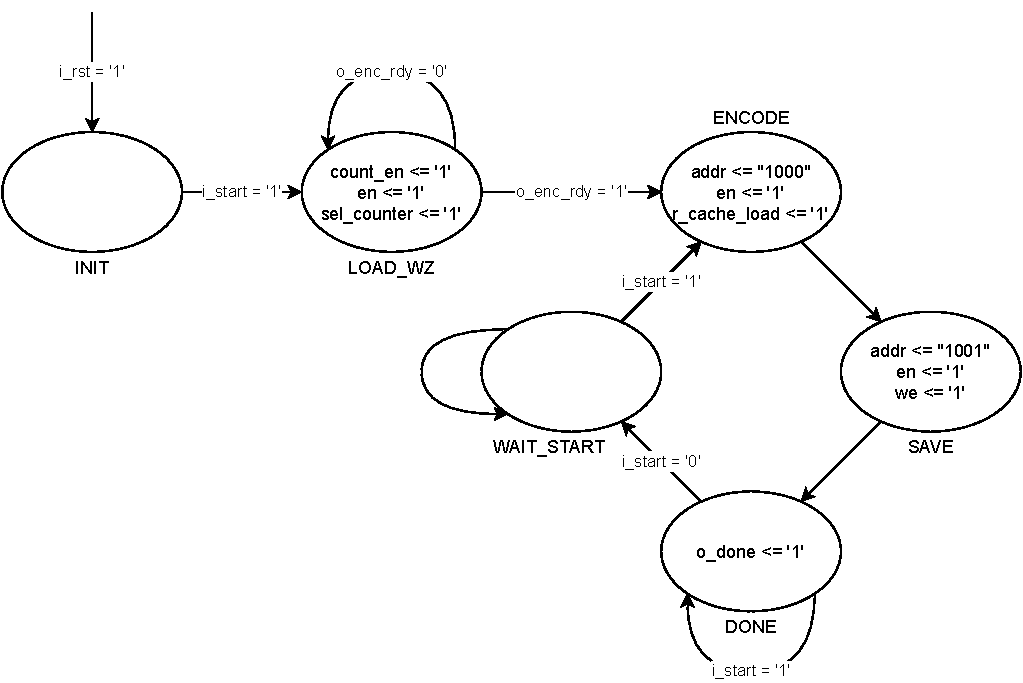
\includegraphics[width=\linewidth]{schema-fsa.pdf}

L'FSA ha 6 stati ed è caratterizzato da due zone di funzionamento, la prima zona è quella iniziale di setup costituita dagli stati `S0' e `S1': una volta ricevuto il segnale di \texttt{i\_start} il componente si prepara alla codifica rimanendo nello stato `S1' mentre sta caricando gli indirizzi delle working zones nei suoi registri interni.

La fine di questa fase è segnalata dal segnale \texttt{o\_enc\_rdy} proveniente dai componenti interni che viene alzato a `1' quando è pronto a codificare, avanzando così l'automa al prossimo stato `S2' e iniziando la fase di codifica.

La fase di codifica iniza nello stato `S2' dove il componente legge l'indirizzo da codificare, lo codifica e lo carica nel registro di cache in un unico ciclo di clock. Nello stato seguente viene scritto in RAM il risultato e in quello dopo viene alzato il segnale di \texttt{o\_done} segnando la fine della codifica.

Dopo di che il componente attenderà l'abbassarsi del segnale di \texttt{i\_start} per abbassare \texttt{o\_done} e poi mettersi in attesa di un nuovo segnale di start nello stato `S5', pronto per una nuova codifica.

\subsection{Moduli interni}
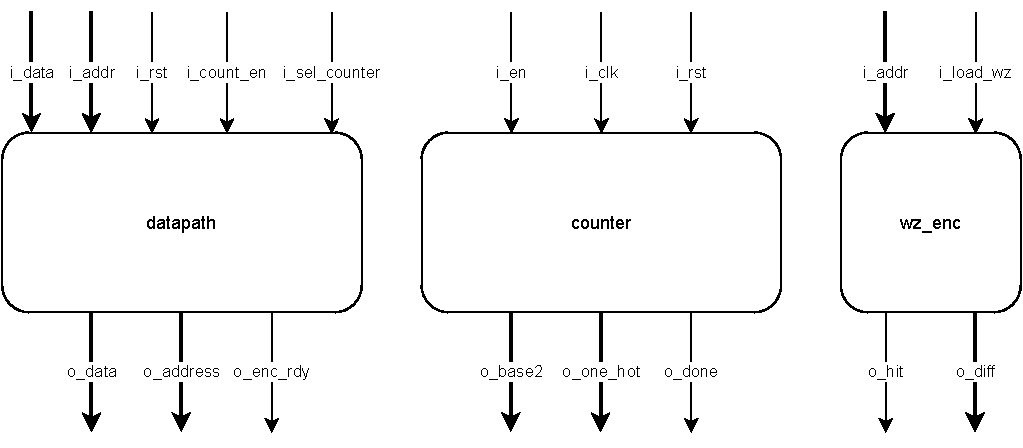
\includegraphics[width=\linewidth]{schema-components.pdf}
Il componente contiene un modulo \texttt{datapath} che ha al suo interno un modulo \texttt{counter} e 8 moduli \texttt{wz\_enc} identici (uno per ogni indirizzo della working zone).

\subsubsection{wz\_enc}
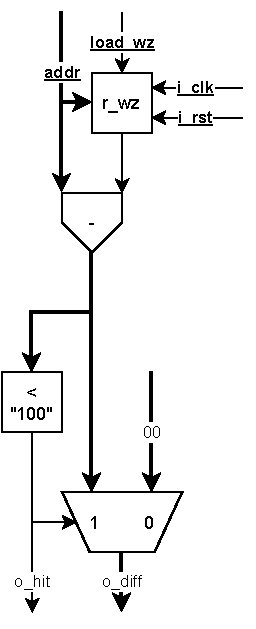
\includegraphics[height=\linewidth]{schema-wz_enc.pdf}

I moduli \texttt{wz\_enc} si occupano di stabilire se un indirizzo sia all'interno di una determinata working zone, segnalandolo con \texttt{o\_hit}, e di calcolarne l'offset in caso positivo. L'offest rispetto alla working zone è \texttt{o\_diff} che è da considerarsi valido solo se \texttt{o\_hit} è a `1', altrimenti avrà tutti i bit a `0'

\subsubsection{counter}

Il modulo \texttt{counter} è un contatore da 0 a 7 che scatta sul falling edge. Esso inizia a contare quando riceve un segnale di enable, dando l'output sia in codifica binaria, sia in codifica one hot, dopo aver sorpassato il 7 tutti i bit degli output vengono messi a `0'

\subsubsection{datapath}
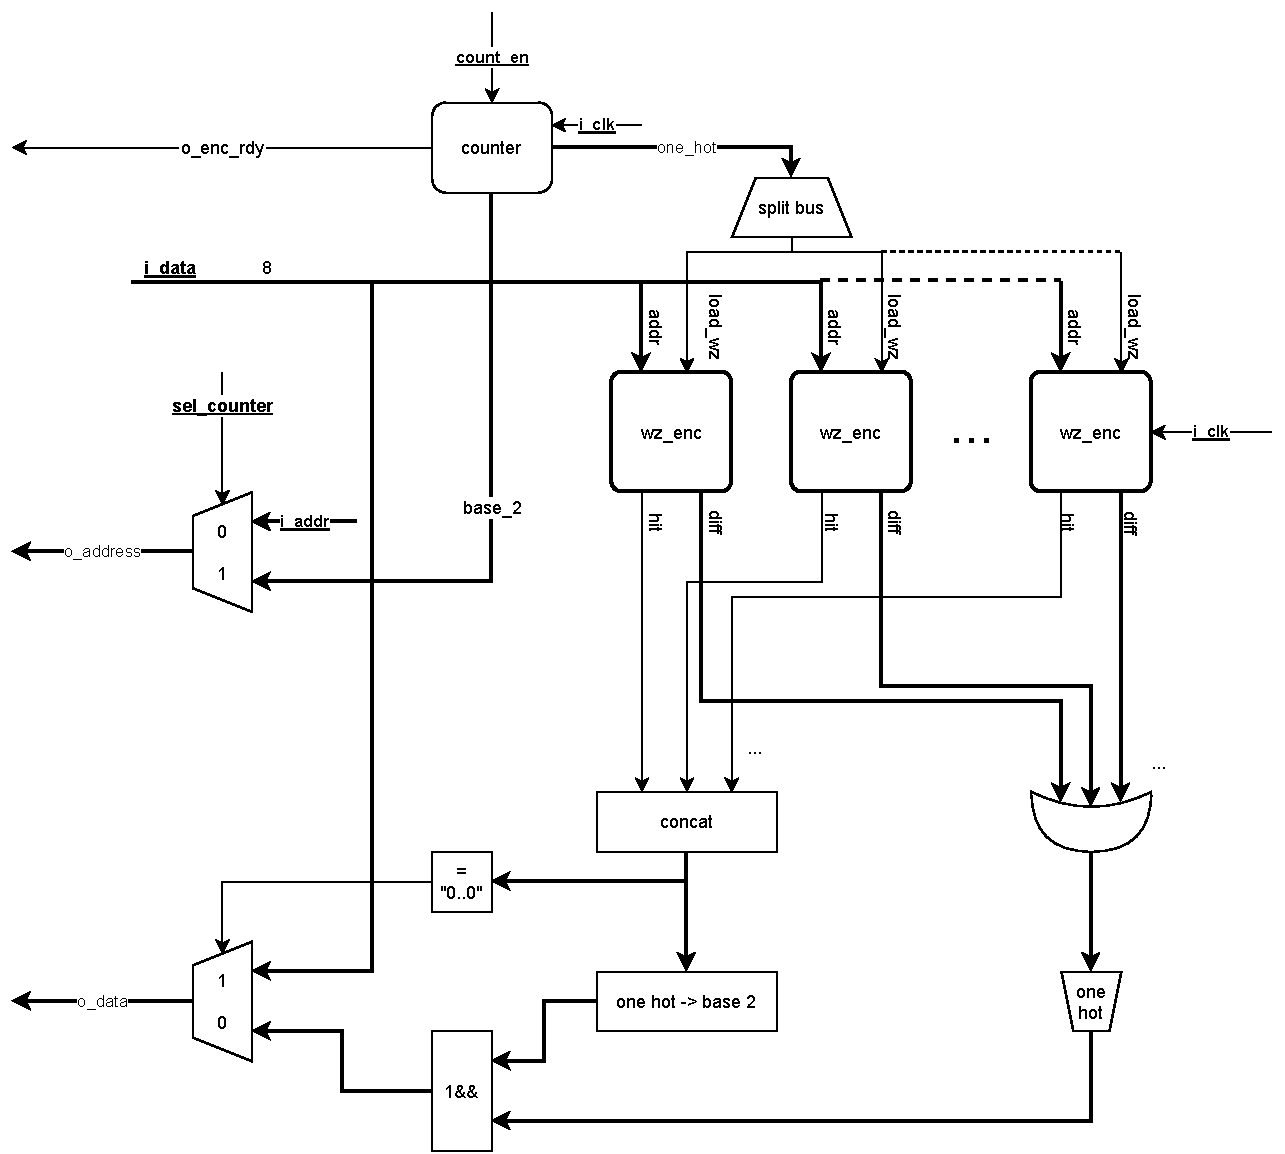
\includegraphics[width=\linewidth]{schema-datapath.pdf}

Il \texttt{datapath} divide il bus contenente la codifica one hot in uscita dal \texttt{counter} collegando ogni bit del segnale al segnale di load di un \texttt{wz\_enc}, in questo modo, usando il segnale in codifica binaria per l'indirizzo in uscita permette di caricare l'indirizzo delle working zone nei rispettivi registri. 

Utilizzando l'output degli \texttt{o\_hit} dei \texttt{wz\_enc} il \texttt{datapath} può rilevare se un indirizzo faccia parte di una working zone o meno, poi combinando gli output degli \texttt{o\_diff} può calcolare la codifica completa dell'indirizzo.


\section{Risultati sperimentali}

Dal report di sintesi si può osservare che il design del componente utilizza in minima parte le risorse disponibili sulla superficie dell'FPGA, non sono presenti black-box e non sono state sintetizzate strutture con un numero di componenti indesiderato.

\hspace{8em}

\begin{tabular}{|p{3.5cm}|c|c|}
\hline
\bf{Site Type}               & \bf{Used}  & \bf{Util\%} \\
\hline
Slice LUTs*             &   98  & 0.07 \\
\hline
  LUT as Logic          &   98  & 0.07 \\
\hline
  LUT as Memory         &    0  & 0.00 \\
\hline
Slice Registers         &   71  & 0.03 \\
\hline
  Register as Flip Flop &   71  & 0.03 \\
\hline
  Register as Latch     &    0  & 0.00 \\
\hline
\end{tabular}

\hspace{8em}

Il numero di nodi utilizzato scala linearmente con il numero di working zone e visto l'ampio margine disponibile sarebbe possibile creare un componente che supporti più working zones con questo stesso design senza incorrere in problemi di eccessiva utilizzazione della superficie dell'FPGA

\hspace{8em}

\begin{tabular}{|p{2cm}|c|p{2.2cm}|}
\hline
\bf{Ref Name}    &   \bf{Used} &  \bf{Functional Category} \\
\hline
FDRE        &     71 &         Flop \& Latch \\
\hline
LUT2        &     58 &                  LUT \\
\hline
OBUF        &     27 &                   IO \\
\hline
LUT4        &     16 &                  LUT \\
\hline
CARRY4      &     16 &           CarryLogic \\
\hline
LUT5        &     15 &                  LUT \\
\hline
LUT6        &     13 &                  LUT \\
\hline
IBUF        &     11 &                   IO \\
\hline
LUT3        &      7 &                  LUT \\
\hline
LUT1        &      1 &                  LUT \\
\hline
BUFG        &      1 &                Clock \\
\hline
\end{tabular}

\hspace{8em}

Primitive utilizzate

\section{Simulazioni}

\section{Conclusioni}

% \end{multicols*}
\end{document}